\documentclass{amsart}
%\documentclass[a4paper,10pt]{scrartcl}

\usepackage[utf8x]{inputenc}
\usepackage[british]{babel}
%\usepackage[a4paper, inner=0.5cm, outer=0.5cm, top=1cm,
%bottom=1.5cm, bindingoffset=1cm]{geometry}
\usepackage{amsmath}
\usepackage{amssymb, latexsym}
\usepackage{longtable}
\usepackage[table]{xcolor}
\usepackage{textcomp} 
\usepackage{graphicx}
\usepackage{enumitem}
\usepackage{hyperref}

\setlist[enumerate]{label*=\arabic*.}
\newtheorem{theorem}{Theorem}[section]
\newtheorem{example}{Example}[section]
\newtheorem{definition}{Definition}[section]
\newtheorem{proposition}{Proposition}[section]
\newtheorem{notation}{Notation}[section]

\title{Blog Post Title}
\author{Henriette Harmse}
\date{\today}

\pdfinfo{%
  /Title    (Blog Post Title)
  /Author   (Henriette Harmse)
  /Creator  ()
  /Producer ()
  /Subject  (DL)
  /Keywords ()
}

\begin{document}
  \maketitle
  \section{First}
  \cite{Aameri2015}

\begin{small}
\begin{verbatim} 
Some code
\end{verbatim}
\end{small}

\begin{figure}
	%trim option's parameter order: left bottom right top
	\centering 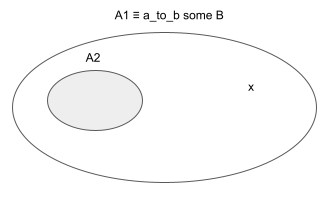
\includegraphics[trim = 0mm 0mm 0mm 0mm, clip, scale=0.9]{./images/EquivalenceVersusSubClassOf-Cropped.png}
	\caption{\texttt{A2} and \texttt{x} wrt \texttt{a\_to\_b some B}}
\end{figure}

\href{http://}{github}
  
  \bibliographystyle{amsplain}
  \bibliography{../../../BibliographicDetails_v.0.1}
 
\end{document}
